Para hacer el modelo utilizamos la notacion vista en la catedra, excepto por las carnalidades donde se representan de manera distinta, asi por ejemplo una relacion M:N sera algo de la forma:

\begin{figure}[ht]
  \begin{center}
    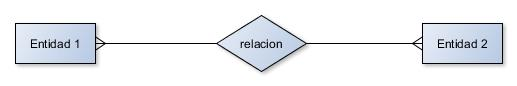
\includegraphics[scale=.75]{ejrelacion.jpg}
    \caption{relacion M:N} 
    \label{fig:graficomn}
  \end{center}
\end{figure}

Una relacion 1 :N sera algo de la forma:

\begin{figure}[ht]
  \begin{center}
    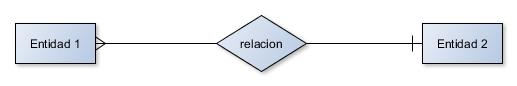
\includegraphics[scale=.75]{ejrelacion2.jpg}
    \caption{relacion N:1} 
    \label{fig:grafico}
  \end{center}
\end{figure}


Aclarado esto procedemos a exhibir el DER.
Separamos el gr�fico en dos fragmentos de manera de hacerlo m�s legible, ambas partes pueden leerse de manera independiente y est�n centradas en la entidad Legislador.

\newpage

\begin{figure}[ht]
  \begin{center}
    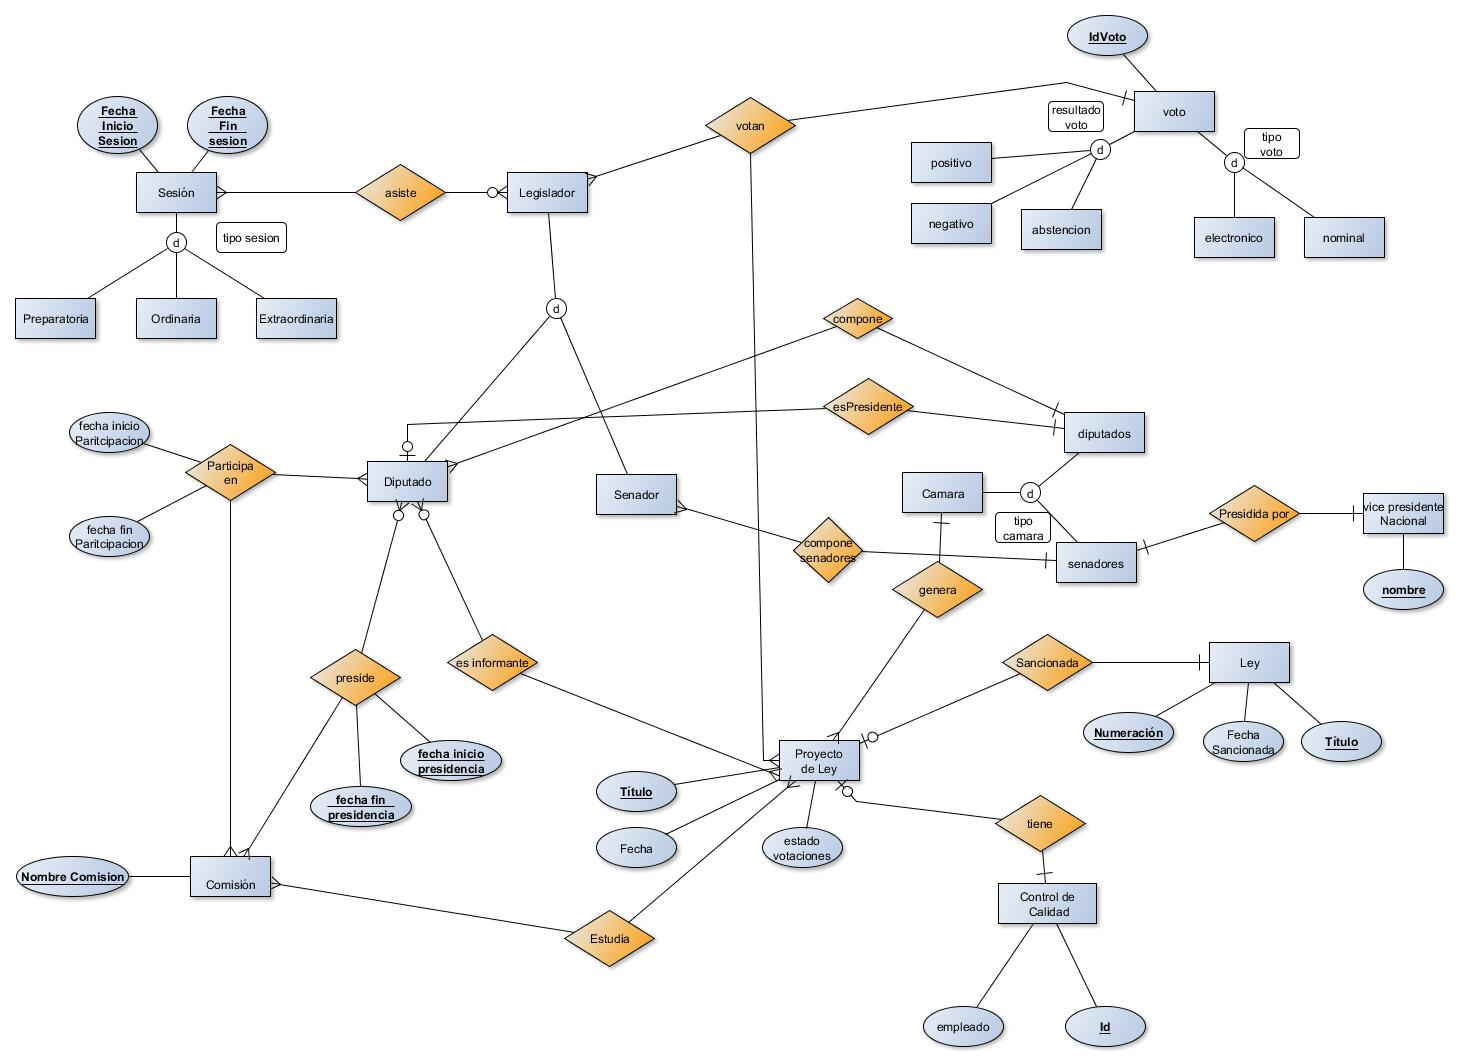
\includegraphics[scale=.50]{DERParteDeAbajo.jpg}
    \caption{fragmento der} 
    \label{fig:derparte1}
  \end{center}
\end{figure}


\newpage

\begin{figure}[ht]
  \begin{center}
    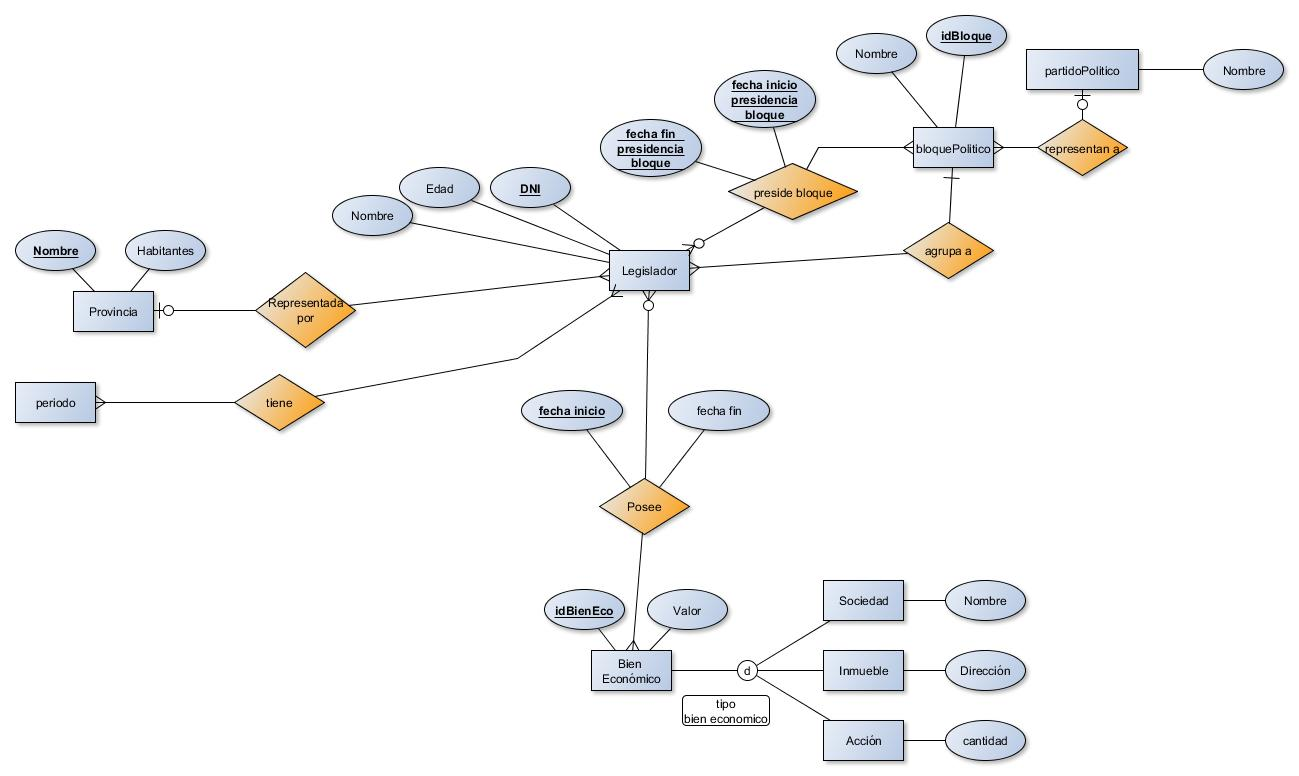
\includegraphics[scale=.50]{DERParteDeArriba.jpg}
    \caption{fragmento der segunda parte} 
    \label{fig:derparte2}
  \end{center}
\end{figure}



